\chapter{Synchrotron Radiation}
\label{cha:synchr-radi}
\index{synchrotron radiation}
Syhchrotron radiation, {\em a.k.a.} magnetic bremmstrahlung, is
produced by relativistic charged particles travelling through a
magnetic field.

\section{Motion in a magnetic field}
\label{sec:moti-magn-field}
\index{motion in a magnetic field}
\index{synchrotron radiation!motion}

The Lorentz force equation relates the rate of change of the
four-momentum to the electric and magnetic field,
\begin{equation}
\dd{p^\mu}{\tau} = \frac{q}{c} F^{\mu\nu} U_\nu
\label{eq:362}
\end{equation}
If the electric field vanishes, we get the following two equations
\begin{equation}
\dd{}{t}(\gamma m {\bf v}) = \frac{q}{c} {\bf v} \times {\bf B}
~\rmmat{and}~
\dd{}{t}(\gamma m c^2) = 0
\label{eq:363}
\end{equation}
The second equation tells us the that the magnitude of the velocity 
does not change.  The first equation tells us that the magnitude of
the velocity ($v_\|$) along the field ${\bf B}$ is also constant.
Because both the magnitude of the velocity and the parallel component
are constant, we find that the magnitude of the perpendicular
component is constant too, so we find
\begin{equation}
\dd{{\bf v}_\perp}{t} = \frac{q}{\gamma m c} {\bf v}_\perp \times {\bf B}
\label{eq:364}
\end{equation}
and the particle gyrates around the magnetic field with a frequency
\begin{equation}
\omega_B = \frac{q B}{\gamma m c}.
\label{eq:365}
\end{equation}
The acceleration ($\omega_B v_\perp$) is perpendicular to the motion
of the particle so we can use formula (44) from Unit 3 to get the
total power, 
\be 
P = \frac{2}{3} \frac{q^2 {\dot u}^2}{c^3} \gamma^4 =
\frac{2q^2}{3c^3} \gamma^2 \frac{q^2 B^2}{m^2 c^2} v^2_\perp =
\frac{2}{3} r_0^2 c \beta^2_\perp \gamma^2 B^2
\label{sec:moti-magn-field-1}\end{equation}
Let's assume that the particles have a random distribution of
velocities relative to the direction of the magnetic field, so we need
the mean value of 
\begin{equation}
\left \langle \beta^2_\perp \right \rangle = \frac{\beta^2}{4\pi} \int
\sin^2\alpha d \Omega = \frac{2\beta^2}{3}
\label{eq:366}
\end{equation}
where $\alpha$ is the pitch angle.

\section{Spectrum of Synchrotron radiation}
\label{sec:spectr-synchr-radi}
\index{synchrotron radiation!spectrum}

If the electron is non-relativistic its dipole moment varies as
$e^{i\omega_B t}$ so we would expect radiation at a single frequency
$\omega_B$.   The relativistic case is somewhat more complicated.
The electron still travels in the circular with a particular frequency
but the electric field essentially vanishes except for a small region
$\Delta \theta \sim 1/\gamma$. near the direction of the electron's
motion (remember relativistic beaming).

We know that the electric field vanishes everywhere except within a cone
of opening angle $1/\gamma$, so a distance observer will only detect a
significant electric field while the electron is within an angle
$\Delta \theta/2 \sim 1/\gamma$ of the point where the path is tangent
to the line of sight.   How long does it take the particle to pass
through this angle?

Using the equation of motion we have
\begin{equation}
\gamma m \frac{\Delta {\bf v}}{\Delta t} = \frac{q}{c} {\bf v} \times
       {\bf B}
\label{eq:367}
\end{equation}
Let's use ${\Delta {\bf v}}=v \Delta \theta=2 v/\gamma$ to get
\begin{eqnarray}
\gamma m \frac{2 v}{\gamma \Delta t} &=& \frac{q}{c} v \sin \alpha B
\\
\Delta t &=& \frac{2 m c}{q B \sin\alpha} = \frac{2}{\gamma \omega_B \sin\alpha}
\label{eq:368}
\end{eqnarray}
We also need to calculate how long between when the radiation emitted
at $t$ and $t+\Delta t$ arrives at the distant observer.   The
difference between the observed times is less than $\Delta t$ by
$v \Delta t/c$ so we get
\begin{equation}
\Delta t^A = \frac{2}{\gamma \omega_B \sin\alpha} \left ( 1 -
\frac{v}{c} \right )
\label{eq:369}
\end{equation}
In the ultrarelativistic limit, $1-v/c \approx 1/(2\gamma^2)$ so we
have
\begin{equation}
\Delta t^A \approx \left ( \gamma^3 \omega_B \sin\alpha \right )^{-1}.
\label{eq:370}
\end{equation}

The distant observer will see zero electric field most of the time
with blips of electric field lasting for a time $\Delta t^A$ every
time the electron loops $2\pi/\omega_B$.   Let's define a critical
frequency,
\begin{equation}
\omega_c \equiv \frac{3}{2} \gamma^3 \omega_B \sin\alpha.
\label{eq:371}
\end{equation}
We expect that the spectrum will cut off at frequencies similar to
$\omega_c$. 

\subsection{Qualitative Spectrum}
\label{sec:qualitative-spectrum}

We earlier found that for a relativistic particle the intensity of the
radiation field depended almost entirely on the combination 
$\gamma\theta$ where $\theta$ is the angle between the line of sight
and the direction of the particle's motion, so
\begin{equation}
E(t) = F(\gamma \theta)
\label{eq:372}
\end{equation}
If we take $t$ to be the
time measured in the observer's frame after $\theta=0$ we find that
\begin{equation}
\gamma\theta \approx 2 \gamma \left ( \gamma^2 \omega_B \sin \alpha
\right) t \propto \omega_c t
\label{eq:373}
\end{equation}
from equation (11), so we find that
\begin{equation}
E(t) = g(\omega_c t).
\label{eq:374}
\end{equation}
To find the spectrum we are interested in Fourier transform of $E(t)$,
\begin{equation}
{\hat E}(\omega) = \frac{1}{2\pi} \int_{-\infty}^\infty
g(\omega_c t) e^{i\omega t} dt. = \frac{1}{2\pi}  \int_{-\infty}^\infty
g(\xi) e^{i\xi \omega/\omega_c} \frac{d\xi}{\omega_c}. = h(\omega/\omega_c)
\label{eq:375}
\end{equation}
so the average power per unit frequency is a function of
$\omega/\omega_c$,
\begin{equation}
\frac{dW}{dtd\omega} = T^{-1} \dd{W}{\omega} \equiv P(\omega) = 
C_1 F\left(\frac{\omega}{\omega_c}\right).
\label{eq:376}
\end{equation}
We already know from equation (5) what the total power emitted by the 
charged particle so we have
\begin{equation}
P = \frac{2}{3} r_0^2 c \beta^2_\perp \gamma^2 B^2 = C_1 \int_0^\infty
F\left(\frac{\omega}{\omega_c}\right) d\omega =  \omega_c C_1 \int_0^\infty
F(x) dx
\label{eq:377}
\end{equation}
We would like the function $F(x)$ to be dimensionless which sets the
value of $C_1$ up to a dimensionless number.  If we take $\beta\approx
1$ we obtain
\begin{equation}
P(\omega) = \frac{\sqrt{3}}{2\pi} \frac{q^3 B \sin\alpha}{mc^2} F\left(\frac{\omega}{\omega_c}\right) 
\label{eq:378}
\end{equation}
where
\begin{equation}
\omega_c = \frac{3\gamma^2 q B \sin\alpha}{2mc}
\label{eq:379}
\end{equation}
\subsection[Power-Law Distribution of Particle Energies]{Spectral Index for a Power-Law Distribution of Particle
\label{sec:spectral-index-power}
  Energies}
\index{synchrotron radiation!non-thermal particles}

Even before calculating the form of $F(\omega/\omega_c)$, we can
determine some interesting properties of the radiation spectrum.
We found from the homework that a shock often gives the electrons that
bounce across it a power-law distribution of energies, such that
\begin{equation}
N(E) dE = C E^{-p} dE~\rmmat{or}~N(\gamma) d\gamma = C \gamma^{-p} d\gamma
\label{eq:380}
\end{equation}
over a particular range of particle energy.  Let's use formula (19) to
calculate the total spectrum from these particles,
\begin{equation}
P_\rmscr{tot} (\omega) = C \int_{\gamma_1}^{\gamma_2} P(\omega) \gamma^{-p}
d\gamma 
\propto \int_{\gamma_1}^{\gamma_2}
F\left(\frac{\omega}{\omega_c}\right) 
\gamma^{-p}d\gamma.
\label{eq:381}
\end{equation}
Let's change variables to $x\equiv \omega/\omega_c$.  Remember that
$\omega_c = A \gamma^2$ so $\gamma^2 \propto \omega/x$, we get
\begin{equation}
P_\rmscr{tot}(\omega) \propto \omega^{-(p-1)/2} \int_{x_1}^{x_2} F(x)
x^{(p-3)/2} d x
\label{eq:382}
\end{equation}
If the range of the power-law distribution is sufficiently large (at
least an order of magnitude) we can take $x_1\rightarrow 0$ and $x_2
\rightarrow \infty$ in (23) so that the integral is simply a constant
and we find that the spectral distribution is also a power-law
$\omega^{-s}$ with a power-law index of $s=(p-1)/2$.  

This power-law spectrum is valid essentially between
$\omega_c(\gamma_1)$ and $\omega_c(\gamma_2)$.  To understand the
spectrum for frequencies outside this range and other details as well
we must calculate the function $F(x)$.

\subsection[Spectrum --- Details]{Spectrum and Polarization of Synchrotron emission ---
\label{sec:spectr-polar-synchr}
  Details}
\index{synchrotron radiation!polarization}
\index{synchrotron radiation!spectrum}

The spectrum of the observed radiation will depend on the Fourier transform
with respect to the observed time of the electric field. The radiation field is
given by the expression
\begin{equation}
{\bf E}(r,t) = \frac{q}{c} \left [ \frac{\bf n}{\kappa^3 R} \times \left [ 
({\bf n} - \betabold ) \times \dot{\betabold} \right ]\right ] 
\ee                              
In chapter three we manipulated this expression under the assumption that we
were really far from the particle so the value of $R$ doesn't change much as
the particle moves to get
\begin{equation}
\frac{d W}{d\omega d\Omega} = \frac{q^2 \omega^2}{4\pi^2 c} 
\left | \int {\bf n} \times ({\bf n} \times \betabold) \exp \left [ i
  \omega \left ( t'-{\bf n} \cdot {\bf r}_0 (t') / c \right ) \right ] dt'
\right |^2
\label{eq:383}
\end{equation}
{
\begin{figure}
{\centering \input sync 
%\includegraphics[width=\textwidth]{syncfig}
}
\caption{Geometry of synchrotron emission}
\end{figure}
}

With no loss of generality we can assume that the particle gyrates in
the $x - y -$plane and our line of sight is in the $x - z -$plane and
makes an angle with the $x-$axis. With this geometric setup we can
calculate 
\begin{equation}
{\bf n} \times ({\bf n} \times \betabold) = -\epbold_\perp \sin \left
( \frac{v t'}{a} \right ) + \epbold_\| \cos \left ( \frac{v t'}{a} \right )
\sin \theta
\label{eq:384}
\end{equation}
The term in the exponential is the observed time in terms of the
retarded time, 
\begin{eqnarray}
t' - \frac{{\bf n} \cdot {\bf r}(t')}{c} &=& t' - \frac{a}{c} \cos
\theta
\sin \left ( \frac{v t'}{a} \right ) \\
&\approx& t' - \frac{a}{c} \left ( 1 - \frac{\theta^2}{2} \right )
\left [ \frac{v t'}{a} - \frac{1}{6} \left ( \frac{v t'}{a} \right )^3
\right ] \\
&\approx& t' - \beta t' + \frac{\theta^2}{2} \beta t' + \frac{c^2
\beta^3 t'^3}{6 a^2} \\
&\approx& \left ( 2 \gamma^2 \right )^{-1} \left [ \left ( 1 +
\gamma^2 \theta^2 \right ) t' + \frac{c^2 \gamma^2 t'^3}{3a^2} \right ]
\label{eq:385}
\end{eqnarray}
To get the final equation we took $1 - \beta \rightarrow
(2\gamma)^{-1}$
and $\beta \rightarrow 1$
.
   Substituting these results into equation (25) and taking the small-angle
approximation for the polarization vectors as well yield
\begin{eqnarray}
\dd{W}{\omega d\Omega} &\equiv& \dd{W_\|}{\omega d\Omega} 
+ \dd{W_\perp}{\omega d\Omega} \\
\dd{W_\perp}{\omega d\Omega} &=& 
\frac{q^2 \omega^2}{4\pi^2 c} \left | 
\int \frac{ct'}{a} \exp \left [ \frac{i\omega}{2\gamma^2} \left (
\theta^2_\gamma t' + \frac{c^2 \gamma^2 t'^3}{3a^2} \right ) \right ]
dt' \right |^2\\
\dd{W_\|}{\omega d\Omega} &=& 
\frac{q^2 \omega^2 \theta^2}{4\pi^2 c} \left | 
\int \exp \left [ \frac{i\omega}{2\gamma^2} \left (
\theta^2_\gamma t' + \frac{c^2 \gamma^2 t'^3}{3a^2} \right ) \right ]
dt' \right |^2
\label{eq:386}
\end{eqnarray}
where $\theta_\gamma^2=1 + \gamma^2 \theta^2$.

Let's make the following change of variables,
\begin{equation}
y \equiv \gamma \frac{c t'}{a \theta_\gamma} ~\rmmat{and}~ \eta \equiv
\frac{\omega a \theta_\gamma^3}{3 c \gamma^3} \approx \frac{\omega}{2\omega_c}
\label{eq:387}
\end{equation}
to yield
\begin{eqnarray}
\dd{W_\perp}{\omega d\Omega} &=& 
\frac{q^2 \omega^2}{4\pi^2 c} 
\left ( \frac{a \theta^2_\gamma}{\gamma^2 c} \right )^2
\left | 
\int_{-\infty}^\infty y \exp \left [ \frac{3}{2} i \eta \left ( y +
\frac{1}{3} y^3 \right ) \right ]
dt' \right |^2\\
\dd{W_\|}{\omega d\Omega} &=& 
\frac{q^2 \omega^2 \theta^2}{4\pi^2 c} 
\left ( \frac{a \theta_\gamma}{\gamma c} \right )^2
\left | 
\int_{-\infty}^\infty y \exp \left [ \frac{3}{2} i \eta \left ( y +
\frac{1}{3} y^3 \right ) \right ]
dt' \right |^2\\
\label{eq:388}
\end{eqnarray}

% \begin{figure}
% \begin{center}
% \includegraphics[width=0.49\columnwidth]{syncct_1}
% \includegraphics[width=0.49\columnwidth]{syncct_5} 

% \includegraphics[width=0.49\columnwidth]{syncct_9}
% \includegraphics[width=0.49\columnwidth]{syncct_99} 
% \end{center}
% \caption{Electric field from a gyrating particle
%  $\beta = 0.1, 0.5, 0.9$ and 0.99.  The insets show the power spectrum
% with $\omega/\omega_c$ along the $x-$axis.  These were calculated
% without the small-angle or ultrarelativistic approximations.  Keep in
% mind a particle with $\gamma=10^3$ has $\beta=0.9999995$.
% }
% \end{figure}

\begin{figure}
\begin{center}
\begin{tikzpicture}
\begin{scope}[yscale=2,xscale=0.4]
\draw plot file{syncmin_0.1} (-3.2,0.6) node {$\beta=0.1$};
\pgftransformxshift{400}
\draw plot file{syncmin_0.5} (-3.6,0.4) node {$\beta=0.5$};
\pgftransformyshift{-40}
\draw plot file{syncmin_0.99} (-4,0.4) node {$\beta=0.99$};
\pgftransformxshift{-400}
\draw plot file{syncmin_0.9} (-4,0.4) node {$\beta=0.9$};
\end{scope}
\begin{scope}[xscale=0.07]
\pgftransformxshift{180}
\pgftransformyshift{25}
\draw plot [yscale=4] file{psync_0.1} ;
\pgftransformxshift{2200}
\draw plot [yscale=20] file{psync_0.5} ;
\pgftransformyshift{-80}
\draw plot [yscale=1000] file{psync_0.99} ;
\pgftransformxshift{-2200}
\draw plot [yscale=100] file{psync_0.9} ;
\end{scope}
\draw [->] (-3.7,-3.2) -- (8,-3.2) node [right] {$t$};
\draw [->] (-3.5,-3.4) -- (-3.5,2) node [above] {$E(t)$};
\end{tikzpicture}
\end{center}
\caption{Electric field from a gyrating particle
 $\beta = 0.1, 0.5, 0.9$ and 0.99.  The insets show the power spectrum
with $\omega/\omega_c$ along the $x-$axis.  These were calculated
without the small-angle or ultrarelativistic approximations.  Keep in
mind a particle with $\gamma=10^3$ has $\beta=0.9999995$.
}
\end{figure}

It turns out that these integrals can be performed with some special
functions called Airy integrals or modified Bessel functions to yield,
\begin{eqnarray}
\dd{W_\perp}{\omega d\Omega} &=& 
\frac{q^2 \omega^2}{4\pi^2 c} 
\left ( \frac{a \theta^2_\gamma}{\gamma^2 c} \right )^2
K^2_\frac{2}{3} (\eta)\\
\dd{W_\|}{\omega d\Omega} &=& 
\frac{q^2 \omega^2 \theta^2}{4\pi^2 c} 
\left ( \frac{a \theta_\gamma}{\gamma c} \right )^2
K^2_\frac{1}{3} (\eta)
\label{eq:389}
\end{eqnarray}

    We would like to find the total emission per orbit over all solid angles.
The emission lies within an angle $1/\gamma$ 
of a cone of half-angle $\alpha$ centered on
the magnetic field, so we can take the element of solid angle 
$d\Omega = 2 \sin \alpha d \theta$
and integrate,
\begin{eqnarray}
\dd{W_\perp}{\omega} &=& 
\frac{2 q^2 \omega^2 a^2 \sin\alpha}{3\pi c^3 \gamma^4}
\int_{-\infty}^\infty
\theta_\gamma^4
K^2_\frac{2}{3} (\eta)
d\theta 
\\
\dd{W_\|}{\omega} &=& 
\frac{2 q^2 \omega^2 a^2 \sin\alpha}{3\pi c^3 \gamma^4}
\int_{-\infty}^\infty
\theta_\gamma^2 \theta^2
K^2_\frac{1}{3} (\eta)
d\theta 
\label{eq:390}
\end{eqnarray}

These integrals can be written in terms of Bessel functions to yield,
\begin{eqnarray}
\dd{W_\perp}{\omega} &=& 
\frac{\sqrt{3} q^2 \gamma \sin\alpha}{2c} \left [ F(x) + G(x) \right ]
\\
\dd{W_\|}{\omega} &=& 
\frac{\sqrt{3} q^2 \gamma \sin\alpha}{2c} \left [ F(x) - G(x) \right ]
\label{eq:391}
\end{eqnarray}
where
\begin{equation}
F(x) = x \int_x^\infty K_\frac{5}{3}(\xi) d\xi, 
~~~~~~~
G(x) = x K_\frac{2}{3}(x)
\label{eq:392}
\end{equation}
and x = $\omega/\omega_c$ .
% \begin{figure}
% \begin{center}
% \begin{tikzpicture}
% \begin{scope}[yscale=3,xscale=2,smooth]
% \draw[very thin,color=gray] (-0.02,-0.02) grid [ystep=0.5] (5.1,1.1);
% \draw[->] (-0.2,0) -- (5.2,0) node[right] {$x$}; 
% \draw[->] (0,-0.2) -- (0,1.2) node[above] {$F(x),G(x)$};
% \draw (0.72,0.9) node {$F(x)$} (1.5,0.25) node {$G(x)$};
% \draw (0,1) node [left] {\small 1};
% \draw (0,0.5) node [left] {\small 0.5};
% \foreach \x in {1,...,5} 
%   \draw (\x,0) node [below] {\small \x};
% \draw[color=red] plot  file{syncf.dat};
% \draw[color=blue] plot file{syncg.dat};
% \end{scope}
% \end{tikzpicture}
% \end{center}
% \caption{Synchrotron Functions}
% \label{fig:fgfunk}
% \end{figure}
\begin{figure}
\begin{center}
\begin{tikzpicture}
\begin{scope}[scale=2.5,smooth]
\clip (-2.5,-3) rectangle (1,2) ;
\draw[color=red] plot file{lsyncf.dat} ;
\draw[color=blue] plot file{lsyncg.dat};
\end{scope}
\begin{scope}[scale=2.5]
\draw[very thin,color=gray] (-2.52,-3.02) grid [ystep=1] (0.7,-0.8);
\draw[->] (-2.7,-3) -- (0.7,-3) node[right] {$x$}; 
\draw[->] (-2.5,-3.2) -- (-2.5,-0.8) node[above] {$F(x),G(x)$};
\draw (-1.8,-1.3) node {$F(x)$} (-1.8,-1.9) node {$G(x)$};
\foreach \x in {-2,...,0} 
  \draw (\x,-3) node [below] {\small $10^{\x}$};
\foreach \x in {-2,...,-1} 
  \draw (-2.5,\x) node [left] {\small $10^{\x}$};
\end{scope}
\end{tikzpicture}
\end{center}
\caption{Synchrotron Functions}
\label{fig:lfgfunk}
\end{figure}

{\bf Something to think about.} Why could we take the limits of integration
in equations (35) and (36) and (39) and (40) to be infinite?

    To convert these values in a power per frequency we have to divide by
the orbital period of the charge $T = 2\pi /\omega_B$ to give
\begin{eqnarray}
P_\perp &=& 
\frac{\sqrt{3} q^3 B \sin\alpha}{4\pi m c^2} \left [ F(x) + G(x) \right ]
\\
P_\| &=& 
\frac{\sqrt{3} q^3 B \sin\alpha}{4\pi m c^2} \left [ F(x) - G(x) \right ]
\label{eq:393}
\end{eqnarray}
The total power is proportional to $F(x)$ that has the following asymptotic
values,
\begin{eqnarray}
F(x) &\sim& \frac{4\pi}{\sqrt{3} \Gamma \left ( \frac{1}{3} \right )}
\left ( \frac{x}{2} \right )^{1/3}, ~~ x \ll\ 1
\label{eq:835} \\
F(x) &\sim& \left(\frac{\pi}{2}\right)^{1/2} e^{-x} x^{1/2}
, ~~ x \gg\ 1 
\label{eq:394}
\end{eqnarray}


\section{Synchrotron Absorption}
\label{sec:synchr-absorpt}

We are particularly interested in the form of the spectrum from a
power-law distribution of particles for frequencies where the region
is optically thick.  We know from the formal soltuion of radiative
transfer that the spectrum approaches the source function at large
optical depth.  Furthermore Eq.~\ref{eq:78} yields a relationship
between the number of particles of various energies and the volume of
phase space at each energy
\begin{equation}
S_\nu = \frac{2h\nu^3}{c^2} \left (
\frac{g_2 n_1}{g_1 n_2} - 1 \right )^{-1}.
\label{eq:838}
\end{equation}
For free ultrarelativistic particles the density of states is
proportional to $E^2$, and we have assumed that their number is
proportional to $E^{-p}$.   Let us imagine that synchrotron emission
is a transition between the upper state at an energy $E+h\nu$ and the
lower state at energy $E$, so
\begin{equation}
\frac{g_2 n_1}{g_1 n_2} - 1 = \frac{(E+h\nu)^2 E^{-p}}{E^2
  (E+h\nu)^{-p}} - 1 = \left ( 1 + \frac{h\nu}{E}\right )^{p+2} - 1
\approx \left ( p + 2 \right ) \frac{h \nu}{E}
\label{eq:840}
\end{equation}
where the final result obtains in the classical limit where $h\nu \ll
E$, so we have
\begin{equation}
S_\nu \approx \frac{2h\nu^3}{c^2} \frac{E}{\left (p+2\right) h \nu}
\approx \frac{2}{\left (p+2\right)} \left ( \frac{4\pi}{3}
  \frac{m^3 c}{q B \sin\alpha} \right )^{1/2} \nu^{5/2}
\label{eq:841}
\end{equation}
where we have related the energy of the state ($E$) to the frequency
through Eq.~\ref{eq:371}.  Notice that the spectral index does not
depend on the power-law index of the particle distribution but rather
results from the power-law relationship between particle energy and
frequency.  Because the optically thin emission spectrum increases
more slowly with frequency than the source function (or even
decreases), we expect synchrotron absorption to be important at low
frequencies where the the integrated optically thin emission exceeds
the source function.


\section{A Complete Synchrotron Spectrum}
 \label{sec:compl-synchr-spectr}
The complete spectrum from synchrotron radiation must account for the
evolution of the electron energies, absorption, the minimum electron
energy and the age of the source.  We have all the necessary
ingredients to figure this out.  First,
\S~\ref{sec:spectral-index-power} calculates the shape of the photon
spectrum for a given power-law distribution of electron energies.
The second ingredient is to calculate the distribution of electron
energies as a function of the time since the electrons were
accelerated (or {\em injected}).   Let us assume that the electrons
initially have a power-law distribution of energies
\begin{equation}
\dd{N}{t d\gamma_0} = C \gamma_0^{-p}  ~\mathrm{for}~\gamma_0>\gamma_m.
\end{equation}
Furthermore the electron energies decrease with time according to
\begin{equation}
\gamma = \frac{\gamma_0 }{1 + A \gamma_0 t'} , A = \frac{2 q^4
  B_\perp^2}{3m^3 c^5}
\label{eq:836}
\end{equation}
where $t'$ is the time since the particles were accelerated
By inverting this equation we obtain the initial electron energy in terms
of the final electron energy
\begin{equation}
  \gamma_0 = \frac{\gamma}{1-A\gamma t'} 
\end{equation}
and
\begin{equation}
   \dd{\gamma_0}{\gamma} = \frac{1}{\left( 1- A \gamma t' \right)^2}
\end{equation}
so
\begin{equation}
\dd{N}{\gamma d t} = C \gamma^{-p} \left ( 1 - A \gamma t' \right )^{p-2}.
\end{equation}
It is crucial to understand the validity of this distribution. Clearly
we must have 
\begin{equation}
\frac{\gamma_m}{1+A\gamma_m t'} < \gamma <
\frac{1}{At'}.
\label{eq:830}
\end{equation}
Otherwise the number of electrons vanishes because either they have
not yet had time to cool to such a low energy or they have already
cooled below this energy.  The original power-law distribution is
truncated at high energies and is extended below $\gamma_m$
by cooling.  

If the source were only active instantaneously or for a short time
long ago $\Delta t \ll t'$, this would be sufficient, but if we are
interested in a source that has been active continually from some time
ago we must intergrate this distribution over the injection times in
the past.  The resulting distribution is 
\begin{equation}
  \dd{N}{\gamma} = C \gamma^{-p} \int_{t_0}^{t_1} \left( 1 - A
  \gamma t'\right )^{p-2} d t' =C \gamma^{-p} \left . \frac{(1 - A
  \gamma t')^{p-1}}{(p-1) (-A\gamma)} \right |_{t_0}^{t_1}
\end{equation}
where the conditions in Eq.~\ref{eq:830} determine the values of $t_0$
and $t_1$.  We have
\begin{equation}
  t_0 = \max\left [0, \frac{1}{A} \left (\gamma^{-1} -
      \gamma_m^{-1} \right ) \right ]~\mathrm{and}~t_1=\min
  \left (t, \frac{1}{A\gamma} \right ).
\label{eq:831}
\end{equation}
The latter expression in Eq.~\ref{eq:831} encourages us to define
\begin{equation}
\gamma_c = \frac{1}{At}.
\end{equation}
We will use this quantity to eliminate $A$ from the equations.
The energy divides the electrons into those that have had a chance to
cool significantly since the source turned on a time $t$ ago and those
that have not cooled significantly.   There are two possibilities for
the resulting distribution depending on whether $\gamma_c$
exceeds $\gamma_m$.  We will examine the distribution for
$\gamma_c>\gamma_m$ first; this is known as the
{\em slow cooling} regime.  There are three possibly ranges for
$\gamma$.  First at the highest energies we have 
\begin{equation}
\dd{N}{\gamma} = \frac{Ct \gamma_c}{p-1} \gamma^{-(p+1)}~\mathrm{for}~\gamma_m< \gamma_c <\gamma.
\label{eq:832}
\end{equation}
For intermediate energies we have
\begin{equation}
\dd{N}{\gamma} = \frac{Ct \gamma_c}{p-1} \gamma^{-(p+1)} \left [ 1 - \left ( 1 - \frac{\gamma}{\gamma_c}
    \right)^{p-1} \right ] ~\mathrm{for}~\gamma_m < \gamma<  \gamma_c 
\label{eq:833}
\end{equation}
For $\gamma \ll\ \gamma_c$ this reduces to
\begin{equation}
\dd{N}{\gamma} \approx  C t \gamma^{-p} ~\mathrm{for}~  \gamma_m < \gamma \ll \gamma_c .
\label{eq:833}
\end{equation}
For the lowest energies the following expression obtains
\begin{equation}
\dd{N}{\gamma} = 
\frac{C t \gamma_c}{p-1} \gamma^{-(p+1)} \left [ \left (\frac{\gamma}{\gamma_m} \right
  )^{p-1} - \left ( 1 - \frac{\gamma}{\gamma_c} \right)^{p-1} \right ]
 ~\mathrm{for}~  \gamma < \gamma_m <  \gamma_c .
\label{eq:834}
\end{equation}

The other cooling regmine is called {\em fast cooling} where
$\gamma_c < \gamma_m$.  Is this regime for the
largest energies $\gamma>\gamma_m>\gamma_c$,
Eq.~\ref{eq:832} also holds.   For intermediate energies we have
\begin{equation}
\dd{N}{\gamma} = \frac{Ct \gamma_c}{(p-1) \gamma_m^{p-1}} \gamma^{-2}~\mathrm{for}~\gamma_c<\gamma<\gamma_m.
\end{equation}
and for the smallest energies
$\gamma<\gamma_c<\gamma_m$ Eq.~\ref{eq:834}
again obtains.

Both of the distributions either for slow or fast cooling vanish for
\begin{equation}
  \gamma < \gamma_\mathrm{cut-off} = \left (
    \frac{1}{\gamma_m} +\frac{1}{\gamma_c}
  \right )^{-1}.
\end{equation}
Well into the slow cooling regime we have $\gamma_m\ll
\gamma_c$ so $\gamma_\mathrm{cut-off} \approx
\gamma_m$.  Well into the fast cooling regime we have
$\gamma_\mathrm{cut-off} \approx \gamma_c$.  To find the
distribution of photon energies we have to convolve the electron
distribution with the function $F(x)$.  
For $\omega > \omega_\mathrm{max}$ where
\begin{equation}
\omega_\mathrm{max} = \frac{3 \gamma_\mathrm{cut-off}^2 q B \sin
  \alpha}{2mc}
\end{equation}
the results of \S~\ref{sec:spectral-index-power} apply.  On the other
hand below this frequency, the radiation results from the
low-frequency limit of the function $F(x)$ (Eq.~\ref{eq:835}),
i.e. $F_\omega \propto \omega^{1/3}$.   A second complication is the
role of synchrotron absorption outlined in
\S~\ref{sec:synchr-absorpt}.   We can combine the various results from
this section to derive a schematic of the emission spectrum from a
synchrotron cooling population of electrons with constant particle
injection.   Figs.~\ref{fig:sync_slow}
and~\ref{fig:sync_fast} depict the spectrum for slow and fast cooling.

% \begin{table}
% \caption{Regimes of Synchrotron Cooling}
% \label{tab:synch-cool}
% \begin{center}
% \begin{tabular}{cccc}
% \hline
% \hline
% Lorentz Factor Range & $dN/d\gamma$ & Frequency Range & $F_\omega$ \\
% \hline
% \multicolumn{4}{c}{\em slow cooling} \\
% \hline
% $\gamma>\gamma_c = \frac{3 m^3 c^5}{2 q^4 B_\perp^2 t}$ &
% $\gamma^{-(p+1)}$ & $\omega > \omega_c=\frac{27}{8} \frac{m^5
%   c^9}{q^7 B_\perp^3 t^2}$ & $F_{\omega,m} \frac{\omega_m^{(p-1)/2} \omega_c^{1/2}}{\omega^{p/2}}$
%  \\
% $\gamma_m < \gamma < \gamma_c$ & \gamma^{-p} & $\omega_m < \omega <
% \omega_c$ & $F_m \left ( \frac{\omega_m}{\omega} \right )^{-(p-1)/2}$ \\
% ? ? & ? & ? ? & ? \\
% ? ? & ? & ? ? & ? \\
% \hline
% \multicolumn{4}{c}{\em fast cooling} \\
% \hline
% ? ? & ? & ? ? & ? \\
% ? ? & ? & ? ? & ? \\
% ? ? & ? & ? ? & ? \\
% ? ? & ? & ? ? & ? \\
% \hline
% \end{tabular}
% \end{center}
% \end{table}

\begin{figure}
\begin{center}
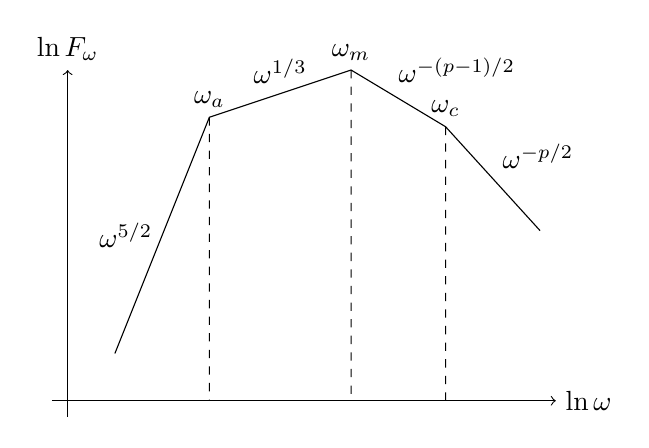
\begin{tikzpicture}
\draw[->] (-0.2,0) -- (6.2,0) node[right] {$\ln \omega$}; 
\draw[->] (0,-0.2) -- (0,4.2) node[above] {$\ln F_\omega$};
\begin{scope}[scale=6]
\draw  (0.1,0.1) -- 
  ++(0.2,0.5) node [above] (oma) {$\omega_a$} 
  node [pos=0.5,left] {$\omega^{5/2}$} -- 
++(0.3,0.1) node [above] (ommi) {$\omega_m$} 
  node [pos=0.5,above] {$\omega^{1/3}$} --
++(0.2,-0.12) node [above] (omc) {$\omega_c$} 
node [pos=0.4,above right] {$\omega^{-(p-1)/2}$} -- 
++(0.2,-0.22) node [pos=0.5,above right] {$\omega^{-p/2}$} ;
\draw [dashed] (oma) -- (0.3,0) (ommi) -- (0.6,0) (omc) -- (0.8,0);
\end{scope}
\end{tikzpicture}
\end{center}
\caption{Complete synchrotron spectrum for an age less than the
  maximum cooling time (slow cooling).}
\label{fig:sync_slow}
\end{figure}

\begin{figure}
\begin{center}
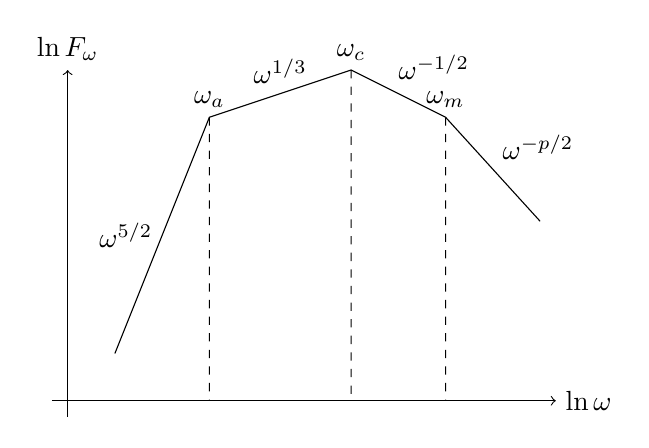
\begin{tikzpicture}
\draw[->] (-0.2,0) -- (6.2,0) node[right] {$\ln \omega$}; 
\draw[->] (0,-0.2) -- (0,4.2) node[above] {$\ln F_\omega$};
\begin{scope}[scale=6]
\draw  (0.1,0.1) -- 
  ++(0.2,0.5) node [above] (oma) {$\omega_a$} 
  node [pos=0.5,left] {$\omega^{5/2}$} -- 
++(0.3,0.1) node [above] (omc) {$\omega_c$} 
  node [pos=0.5,above] {$\omega^{1/3}$} --
++(0.2,-0.1) node [above] (ommi) {$\omega_m$} 
node [pos=0.4,above right] {$\omega^{-1/2}$} -- 
++(0.2,-0.22) node [pos=0.5,above right] {$\omega^{-p/2}$} ;
\draw [dashed] (oma) -- (0.3,0) (omc) -- (0.6,0) (ommi) -- (0.8,0);
\end{scope}
\end{tikzpicture}
\end{center}
\caption{Complete synchrotron spectrum for an age greater than the
  maximum cooling time (fast cooling).}
\label{fig:sync_fast}
\end{figure}

To learn more about the frequency spectrum of synchrotron emission
from mono-energetic electrons, consult Chapter \S14.6
of
\begin{itemize}
\item Jackson, J. D., {\em Classical Electrodynamics}.
\end{itemize}

\section{Problems}
\begin{enumerate}
\item{\bf Synchrotron Radiation:}

An ultrarelativistic electron emits synchrotron radiation.  Show that
its energy decreases with time according to
\begin{equation}
\gamma = \gamma_0 \left ( 1 + A \gamma_0 t \right )^{-1}, A=\frac{2e^4
  B_\perp^2}{3m^3 c^5}.
\label{eq:395}
\end{equation}
Here $\gamma_0$ is the initial value of $\gamma$ and $B_\perp = B
\sin\alpha$.  Show that the time for the electron to lose half its
energy is
\begin{equation}
t_{1/2} = \left (A\gamma_0\right)^{-1}
\label{eq:396}
\end{equation}
How do you reconcile the decrease of $\gamma$ with the result of
constant $\gamma$ for motion in a magnetic field?

\item{\bf Synchrotron Cooling More Precisely:}

Derive the evolution of the energy of the electron (or $\gamma$)
evolves in time without making the ultrarelativistic approximation.

\item{\bf Power-Law Distribution More Precisely:}

Calculate the photon spectrum for a power-law distribution of electron
energies as in \S~\ref{sec:spectral-index-power} including the
normalization and polarization. 

\end{enumerate}
%%% Local Variables:
%%% TeX-master: "book"
%%% End:
